\documentclass[11pt,a4paper]{article}
\usepackage[margin=1.0in]{geometry}
\usepackage[skip=8pt plus1pt, indent=0pt]{parskip}
\usepackage[scaled]{berasans}
\renewcommand*\familydefault{\sfdefault}

\usepackage{polski}
\usepackage[T1]{fontenc}
\usepackage[utf8]{inputenc}

\usepackage{hyperref}
\usepackage{amsmath, amsthm}
\usepackage{graphicx}
\usepackage{float}

\usepackage[color=orange!25]{todonotes}
\usepackage{listings}
\newcommand{\todoinfo}[2][]{\todo[color=green!30, #1]{#2}}
\newcommand{\deemph}[1]{{\color{black!40}{\footnotesize #1}}}


\title{Raport z laboratorium przedmiotu\\Informatyka w Medycynie\\Projekt tomografu}
\author{\emph{Ivan Kaliadzich 153936, Mikołaj Diakowski 151843}}
\date{24 marca 2024}


\begin{document}
\maketitle
    \section{Zastosowany model tomografu}
    W projekcie zdecydowaliśmy się na zastosowanie modelu tomografu
    \section{Zastosowany język programowania wraz z bibliotekami}
    W projekcie użyliśmy następujących bibliotek:
    \begin{itemize}
        \item \texttt{imageio} - do wczytywania obrazów
        \item \texttt{ipywidgets} - do tworzenia interaktywnych elementów
        \item \texttt{numpy} - do operacji matematycznych
        \item \texttt{pydicom} - do wczytywania obrazów w formacie DICOM
        \item \texttt{matplotlib} - do rysowania wykresów
        \item \texttt{scipy} - do przetwarzania sygnałów
        \item \texttt{skimage} - do przetwarzania obrazów
        \end{itemize}
    \section{Opis głównych funkcji programu}
    \subsection{Pozyskiwanie odczytów dla poszczególnych detektorów}
    Fragment kodu:
\begin{lstlisting}[language=Python, basicstyle=\normal, breaklines=true]
photo = imageio.imread('SADDLE_PE.JPG', mode = 'F')

plt.figure(figsize=(16,16))
plt.subplots_adjust(wspace=0.2)
sub1 = plt.subplot(131)
sub1.set_title("Obraz wejściowy")
sub1.set_xticks([],[])
sub1.set_yticks([],[])
sub1.imshow(photo, cmap='gray')


sinogram = radon_transform(photo, d_a, range_pi, n_detect, d_x)

xlabels=[i*20 for i in range(10)]
sub2 = plt.subplot(132)
sub2.set_xticks(np.arange(0, 181/d_x, 20/d_x))
sub2.set_xticklabels(xlabels)
sub2.set_xlabel("Kąt projekcji")
sub2.set_title("Sinogram")
sub2.imshow(sinogram, cmap='gray')


if filter == True:
    sinogram2 = filtration(sinogram)
else:
    sinogram2 = sinogram
constr, projection = back_projection(sinogram2, d_x)

sub3 = plt.subplot(133)
sub3.set_title("Obraz wyjściowy")
sub3.set_xticks([],[])
sub3.set_yticks([],[])
sub3.imshow(constr, cmap='gray')
    \end{lstlisting}
    Na początku wczytujemy obraz wejściowy, następnie przeprowadzamy na nim transformację Radona.
    Następnie przeprowadzamy filtrację, jeśli jest taka potrzeba.
    Na końcu przeprowadzamy odwrotną transformację Radona.
    \subsection{Filtracja sinogramu i zastosowany rozmiar maski}
\begin{lstlisting}[language=Python, basicstyle=\normal, breaklines=true]
def filtration(sinogram):
    h = np.array([[-1,-1,-1],[-1,9,-1],[-1,-1,-1],], dtype = 'float')
    filter_photo = signal.convolve2d(sinogram,h)
    filter_photo=filter_photo[2:-2,2:-2]
    return filter_photo
\end{lstlisting}
    Maska użyta w tej funkcji to tzw.
    maska Laplace'a, która jest często używana do wykrywania krawędzi w obrazach.
    W naszym przypadku maska ta służy do wyostrzenia obrazu.
    \subsection{Ustalanie jasności poszczególnych punktów obrazu wynikowego oraz jego przetwarzanie końcowe}

\begin{lstlisting}[language=Python, basicstyle=\normal, breaklines=true]
def radon_transform(photo, d_a, range_pi, detectors_number, d_x):
    alfa = math.pi / 2
    n = math.ceil(180 /d_x) + 1
    detectors = [[0,0] for _ in range(detectors_number)]
    emiters = [[0,0] for _ in range(detectors_number)]
    length = len(photo)
    width = len(photo[0])
    r = math.floor(math.sqrt(length*length+width*width)/2)

    photo1 = [[0 for _ in range(r*2)] for __ in range(r*2)]
    l, w = photo.shape
    y_off = round((r * 2 - l)/2)
    x_off = round((r * 2 - w)/2)
    photo1= np.array(photo1.copy())
    photo1[y_off:y_off+l, x_off:x_off+w] = photo

    sinogram=[]

    for i in range(n):
        str = [0 for _ in range(detectors_number)]
        for j in range(detectors_number):
            x = r * math.cos(alfa + math.pi - (1/2) * range_pi + j * (range_pi / (detectors_number - 1)) + (i * d_a))
            y = r * math.sin(alfa + math.pi - (1/2) * range_pi + j * (range_pi / (detectors_number - 1)) + (i * d_a))

            detectors[j] = [round(x), round(y)]
            x_e  = r*math.cos(alfa + (1/2) * range_pi - j * (range_pi / (detectors_number - 1)) + (i * d_a))
            y_e = r*math.sin(alfa + (1/2) * range_pi - j * (range_pi / (detectors_number - 1)) + (i * d_a))
            emiters[j]=[round(x_e),round(y_e)]
            points = bresenham_algorithm(emiters[j][0], emiters[j][1], detectors[j][0], detectors[j][1])
            k =1

            for x_p ,y_p in points:
                if x_off < x_p + r < x_off + w and y_off < y_p + r < y_off + l:
                    str[j] += photo1[x_p + r - 1][y_p + r - 1]
                    k+=1

            if k > 1:
                k -= 1
            str[j] /= k

        sinogram.append(str)

    sinogram = np.rot90(sinogram, 1, axes=(0,1))
    return sinogram
\end{lstlisting}
    Funkcja ta przeprowadza transformację Radona na obrazie wejściowym.
    Algorytm ten pozwala jednocześnie na uśrednienie jasności punktów obrazu wynikowego, a także na jego normalizację.
    \subsection{Wyznaczanie wartości miary RMSE na podstawie obrazu źródłowego oraz wynikowego}\label{sec:wyznaczanie-wartosci-miary-rmse-na-podstawie-obrazu-zrodowego-oraz-wynikowego}
    \begin{lstlisting}[language=Python, basicstyle=\normal, breaklines=true]
def calculate_mse(image1, image2):
    return mean_squared_error(image1, image2)

def analyze_mse(original_image):
    # List to store MSE values
    mse_values = []
    detectors_number = 180

    for i in range(1, 181):
        radon_image = radon_transform(original_image, d_a, range_pi, detectors_number, d_x)
        reconstructed_image = back_projection(radon_image, d_x)
        mse = calculate_mse(original_image, reconstructed_image)
        mse_values.append(mse)

    return mse_values

def analyze_mse_sampling(original_image):
    mse_values_sampling = []

    for i in range(1, 181):
        radon_image = radon_transform(original_image, d_a * i, range_pi * i, n_detect * i, d_x)
        reconstructed_image = back_projection(radon_image, d_x)
        mse = calculate_mse(original_image, reconstructed_image)
        mse_values_sampling.append(mse)

    return mse_values_sampling

def analyze_mse_filtering(original_image, theta):
    mse_values_filtering = []

    for i in range(1, 181):
        radon_image = radon_transform(original_image, d_a, range_pi, n_detect, d_x)
        reconstructed_image = back_projection(filtration(radon_image), d_x)
        mse = calculate_mse(original_image, reconstructed_image)
        mse_values_filtering.append(mse)

    return mse_values_filtering
\end{lstlisting}
    Funkcja \texttt{calculate\_mse} oblicza wartość miary RMSE dla dwóch obrazów.
    Wewnątrz wykorzystujemy gotową implementację z biblioteki \texttt{skimage}: \texttt{mean\_squared\_error}.

    \subsection{Odczyt i zapis plików DICOM}
    \begin{lstlisting}[language=Python, basicstyle=\normal, breaklines=true]
def open_dicom(name_dcm):
    information = pydicom.dcmread(name_dcm, force=True)
    name_patient = information.PatientName
    date_patient = information.StudyDate
    commentary_patient = information.StudyDescription
    print("Informacje")
    print("Imie i nazwisko: ", name_patient)
    print("Data: ", date_patient)
    print("Komentarz: ", commentary_patient)
    plt.imshow(information.pixel_array,cmap="gray")

def create_dicom(name_patient, date_patient, commentary_patient):
    global constr_new
    photo_dcm = (constr_new).astype(np.uint16)

    meta = pydicom.Dataset()
    meta.MediaStorageSOPClassUID = pydicom._storage_sopclass_uids.MRImageStorage
    meta.MediaStorageSOPInstanceUID = pydicom.uid.generate_uid()
    meta.TransferSyntaxUID = pydicom.uid.ExplicitVRLittleEndian

    Data = pydicom.Dataset()
    Data.file_meta = meta
    Data.is_little_endian = True
    Data.is_implicit_VR = False
    Data.SOPClassUID = pydicom._storage_sopclass_uids.MRImageStorage
    Data.PatientName = name_patient
    Data.StudyDate = date_patient
    Data.StudyDescription = commentary_patient
    Data.Modality = "MR"
    Data.SeriesInstanceUID = pydicom.uid.generate_uid()
    Data.StudyInstanceUID = pydicom.uid.generate_uid()
    Data.FrameOfReferenceUID = pydicom.uid.generate_uid()

    Data.BitsAllocated = 16
    Data.BitsStored = 16
    Data.HighBit = 15
    Data.SamplesPerPixel = 1
    Data.ImagesInAcquisition = "1"
    Data.Rows = photo_dcm.shape[0]
    Data.Columns = photo_dcm.shape[1]

    Data.ImagePositionPatient = r"0\0\1"
    Data.ImageOrientationPatient = r"1\0\0\0\-1\0"
    Data.ImageType = r"ORIGINAL\PRIMARY\AXIAL"
    Data.RescaleIntercept = "0"
    Data.RescaleSlope = "1"
    Data.PixelSpacing = r"1\1"
    Data.PhotometricInterpretation = "MONOCHROME2"
    Data.PixelRepresentation = 1

    pydicom.dataset.validate_file_meta(Data.file_meta, enforce_standard=True)
    Data.PixelData = photo_dcm.tobytes()
    Data.save_as("DICOM.dcm")
    \end{lstlisting}
    Funkcja \texttt{create\_dicom} tworzy plik DICOM na podstawie obrazu wynikowego.
    Funkcja \texttt{open\_dicom} odczytuje plik DICOM i wyświetla informacje o pacjencie oraz obraz.

    \subsection{Przykładowy wynik działania programu}
    \begin{figure}[H]
        \centering
        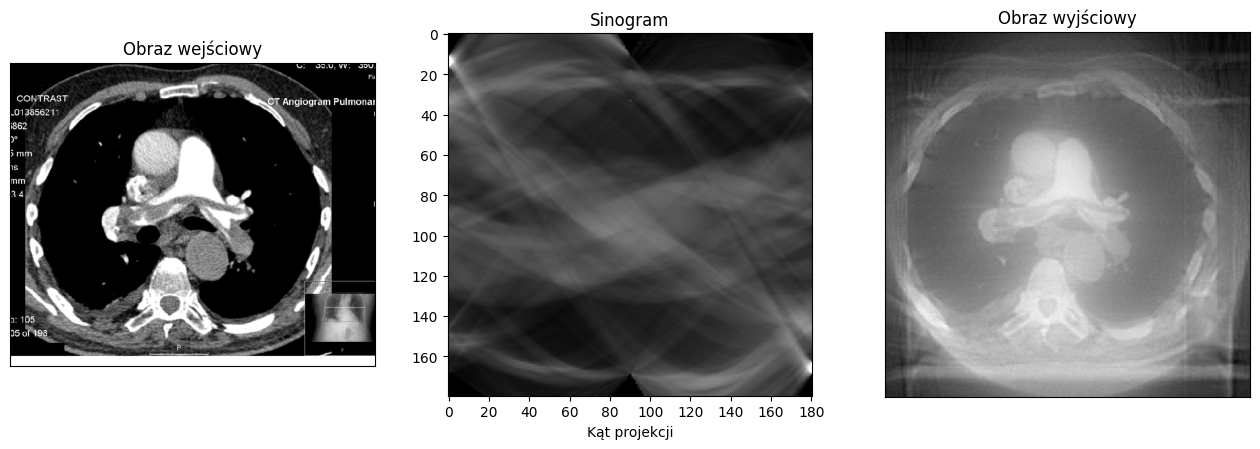
\includegraphics[width=0.8\textwidth]{inputoutput1}
        \caption{Przykładowy wynik działania programu}
    \end{figure}
\end{document}